\documentclass{article}
\usepackage{graphicx} % Required for inserting images
\usepackage[margin=1in]{geometry}
\usepackage{bm, amsfonts, amsmath, tikz, pgfplots}
\pgfplotsset{compat=newest, width=10cm}

\usetikzlibrary{external}
\tikzexternalize[prefix=TikzPictures]

\title{32AH Notes}
\author{Brendan Connelly}
\date{December 2023}

\newcommand{\R}{\mathbb{R}}
\newcommand{\C}{\mathbb{C}}
\newcommand{\Z}{\mathbb{Z}}
\newcommand{\Q}{\mathbb{Q}}
\newcommand{\F}{\mathbb{F}}

\begin{document}

\maketitle

\section*{Linear Algebra}

\textbf{Vector Space Axioms}

\begin{enumerate}
    \renewcommand{\labelenumi}{\roman{enumi}}
    \item Additive Associativity: $\bm{u} + (\bm{v} + \bm{w}) = (\bm{u} + \bm{v}) + \bm{w}$
    \item Additive Identity: $\bm{v} + \bm{0} = \bm{0} + \bm{v} = \bm{v}$
    \item Additive Inverse: \textit{For all $\bm{v} \in V$ there exists a  $\bm{w} \in V$ such that $\bm{v} + \bm{w} = \bm{0}$}
    \item Additive Commutativity: $\bm{u} + \bm{v} = \bm{v} + \bm{u}$
    \item Scalar Associativity: $\lambda \left(\alpha \bm{v} \right) = \left(\lambda \alpha \right) \bm{v}$
    \item Scalar Identity: $1\bm{v} = \bm{v}$
    \item Distribution of Scalar Addition: $\left( \lambda + \alpha \right) \bm{u} = \lambda \bm{u} + \alpha \bm{u}$
    \item Distribution of Vector Addition: $\lambda \left( \bm{u} + \bm{v} \right) = \lambda \bm{u} + \lambda \bm{v}$
\end{enumerate}

\vspace{0.5cm}

\noindent \textbf{Vector Subspace}

\begin{enumerate}
    \renewcommand{\labelenumi}{\roman{enumi}}
    \item Non-empty $\Rightarrow$ contains the zero vector
    \item Closed under vector addition $\Rightarrow \bm{u} + \bm{v} \in W$
    \item Closed under scalar multiplication $\Rightarrow \lambda (\bm{v}) \in W$
\end{enumerate}

\vspace{0.5cm}

\noindent \textbf{Pointwise addition and scalar multiplication of continuous functions $f: \R \to \R$}

\begin{enumerate}
    \renewcommand{\labelenumi}{\roman{enumi}}
    \item $(f + g)(x) := f(x) + g(x)$
    \item $(\lambda f)(x) := \lambda (f(x))$
\end{enumerate}

\vspace{0.5cm}

\noindent \textbf{Basis of a Vector Space}

\textit{An ordered set of vectors $B$ is a basis of $V$ if}

\begin{enumerate}
    \renewcommand{\labelenumi}{\roman{enumi}}
    \item $\mathcal{B} \subset$ V
    \item span($\mathcal{B}$) = V
    \item $\mathcal{B}$ is linearly independent
\end{enumerate}

\vspace{0.5cm}

\noindent \textbf{Linear Independence/Dependence}

\textit{A set of vectors $A \subset V$ is said to be linearly dependent if for every nonempty finite subset of vectors $\{ \bm{v}_1, \ldots , \bm{v}_k \} \subset A$, there exist scalars $\alpha_i$, \underline{not all zero}, such that}

$$\alpha_i \bm{v}_i + \ldots + \alpha_k \bm{v}_k = \bm{0}$$

\textit{Otherwise, the set of vectors $A$ is linearly independent}

\vspace{0.5cm}

\noindent \textbf{Linear Maps}

A linear map $T:V \to W $ is defined as follows for all $k \in \mathbb{N}, \alpha_{i} \in \R$, and all vectors $x_i \in V$

$$T\left(\sum\limits_{i}^{k}\alpha_{i}x_{i}\right) = \sum\limits_{i}^{k}\alpha_{i}T(x_{i})$$

Equivalently, a linear map will satisfy the following:

\begin{enumerate}
    \renewcommand{\labelenumi}{\roman{enumi}}
    \item $T(\bm{u} + \bm{v}) = T(\bm{u}) + T(\bm{v})$
    \item $T(\lambda \bm{u}) = \lambda T(\bm{u})$
\end{enumerate}

\vspace{0.5cm}

\noindent \textbf{Standard Matrix}

Given a basis $\mathcal{B} = \{ \bm{e_1}, \ldots ,\bm{e_n} \} $, the standard matrix $A$ of a linear map $T: \R^n \to \R^m$ is given by 

$$\begin{bmatrix} A \end{bmatrix} = \begin{bmatrix}
| & | & & | \\
T(e_1) & T(e_2) & \cdots & T(e_n) \\
| & | & & |
\end{bmatrix} \in M_{m \times n} (\R)$$

\vspace{0.5cm}

\noindent \textbf{Determinant Formulas}

$$\begin{vmatrix}
a & b \\
c & d \\
\end{vmatrix}
= ad - bc $$

$$\begin{vmatrix}
a_1 & b_1 & c_1 \\
a_2 & b_2 & c_2 \\
a_3 & b_3 & c_3 \\
\end{vmatrix}
= a_1 \begin{vmatrix} b_2 & c_2 \\ b_3 & c_3 \end{vmatrix}
- b_1 \begin{vmatrix} a_2 & c_2 \\ a_3 & c_3 \end{vmatrix}
+ c_1 \begin{vmatrix} a_2 & b_2 \\ a_3 & b_3 \end{vmatrix}
$$

\vspace{0.5cm}

\noindent \textbf{Inverse of a matrix $\in M_{2 \times 2} (\R)$}

$$\begin{bmatrix}
a & b \\
c & d \\
\end{bmatrix}^{-1}
= \frac{1}{ad - bc}
\begin{bmatrix}
d & -b \\
-c & a \\
\end{bmatrix}
$$

\vspace{0.5cm}

\noindent \textbf{Dot Product}

The dot product of two vectors can be defined in two primary ways:

\begin{enumerate}
    \item \textbf{Algebraic Definition:} \\
    Given two vectors \( \bm{a} = (a_1, a_2, \ldots, a_n) \) and \( \bm{b} = (b_1, b_2, \ldots, b_n) \) in an n-dimensional space, their dot product is the sum of the products of their corresponding components:
    \[ \bm{a} \cdot \bm{b} = a_1b_1 + a_2b_2 + \ldots + a_nb_n \]

    \item \textbf{Geometric Definition:} \\
    The dot product of two vectors \( \bm{a} \) and \( \bm{b} \) can also be defined as the product of their magnitudes and the cosine of the angle \( \theta \) between them:
    \[ \bm{a} \cdot \bm{b} = \|\bm{a}\| \|\bm{b}\| \cos \theta \]
    where \( \|\bm{a}\| \) and \( \|\bm{b}\| \) are the magnitudes of vectors \( \bm{a} \) and \( \bm{b} \), respectively.
\end{enumerate}

\vspace{0.5cm}

\noindent \textbf{Cross Product}

The cross product of two vectors in three-dimensional space can be defined in three ways:

\begin{enumerate}
    \item \textbf{Determinant Definition:} \\
    Given two vectors \( \bm{a} = (a_1, a_2, a_3) \) and \( \bm{b} = (b_1, b_2, b_3) \), their cross product can be expressed using the determinant of a matrix:
    \[ \bm{a} \times \bm{b} = \begin{vmatrix}
    \hat{i} & \hat{j} & \hat{k} \\
    a_1 & a_2 & a_3 \\
    b_1 & b_2 & b_3
    \end{vmatrix} \]
    where \( \hat{i}, \hat{j}, \hat{k} \) are the unit vectors in the direction of the x, y, and z axes, respectively.

    \item \textbf{Magnitude and Direction Definition:} \\
    The magnitude of the cross product is given by the product of the magnitudes of the two vectors and the sine of the angle \( \theta \) between them:
    \[ \|\bm{a} \times \bm{b}\| = \|\bm{a}\| \|\bm{b}\| \sin \theta \]
    The direction of \( \bm{a} \times \bm{b} \) is perpendicular to the plane formed by \( \bm{a} \) and \( \bm{b} \), following the right-hand rule.

    \item \textbf{Algebraic Definition:} \\
    Given two vectors \( \bm{u}, \bm{v} \in \mathbb{R}^3 \), their cross product \( \bm{u} \times \bm{v} \) is the unique vector in \( \mathbb{R}^3 \) defined by the property:
    \[ (\bm{u} \times \bm{v}) \cdot \bm{w} = \det \begin{bmatrix} \bm{u} \\ \bm{v} \\ \bm{w} \end{bmatrix} \]
    for all \( \bm{w} \in \mathbb{R}^3 \).
\end{enumerate}

\vspace{0.5cm}

\begin{minipage}[t]{0.5\textwidth}
\textbf{Properties of the Dot Product:}

\begin{enumerate}
    \item \( \bm{u} \cdot \bm{v} = \bm{v} \cdot \bm{u} \) (Commutativity).
    \item \( \lambda(\bm{u} \cdot \bm{v}) = (\lambda \bm{u}) \cdot \bm{v} = \bm{u} \cdot \lambda(\bm{v}) \) (Compatibility with Scalars).
    \item \( \bm{u} \cdot (\bm{v} + \bm{w}) = \bm{u} \cdot \bm{v} + \bm{u} \cdot \bm{w} \) (Distribution).
    \item \( \bm{v} \cdot \bm{v} \geq 0 \), equality only when \( \bm{v} = \bm{0} \) (Positive Definite).
    \item Cauchy-Schwarz Inequality: \( |\bm{u} \cdot \bm{v}| \leq \|\bm{u}\| \|\bm{v}\| \).
    \item Triangle Inequality: \( \|\bm{u} + \bm{v}\| \leq \|\bm{u}\| + \|\bm{v}\| \).
\end{enumerate}
\end{minipage}
\hfill
\begin{minipage}[t]{0.5\textwidth}
\textbf{Properties of the Cross Product:}

\begin{enumerate}
    \item \( \bm{u} \times \bm{v} = -(\bm{v} \times \bm{u}) \) (Anti-commutativity).
    \item \( \bm{u} \times \bm{v} \) is orthogonal to both \( \bm{u} \) and \( \bm{v} \).
    \item The cross product \( \times : \mathbb{R}^3 \rightarrow \mathbb{R}^3 \rightarrow \mathbb{R}^3 \) is bilinear.
    \item \( \bm{u} \times \bm{v} = \bm{0} \) if and only if \( \bm{u} \) and \( \bm{v} \) are parallel.
\end{enumerate}
\end{minipage}

\vspace{0.5cm}

\noindent \textbf{Orthogonal/Orthonormal}

A subset of vectors \( S = \{v_1, v_2, \ldots, v_k\} \subseteq \mathbb{R}^n \) is said to be orthogonal if
\[ v_i \cdot v_j = 0 \quad \text{for all } i \neq j. \]

Furthermore, if \( \|v_i\| = 1 \) for all \( 1 \leq i \leq k \), we say that the subset \( S = \{v_1, v_2, \ldots, v_k\} \subseteq \mathbb{R}^n \)
is orthonormal.

\vspace{0.5cm}

\noindent \textbf{Projection of a \( \bm{u}\) along a \( \bm{v}\)}

Assume \( \bm{v} \neq 0 \). The projection of \( \bm{u} \) along \( \bm{v} \) is the vector
\[ \bm{u}_{\parallel \bm{v}} = \left( \frac{\bm{u} \cdot \bm{v}}{\bm{v} \cdot \bm{v}} \right) \bm{v} = \left( \frac{\bm{u} \cdot \bm{v}}{\|\bm{v}\|^2} \right) \bm{v} = \left( \frac{\bm{u} \cdot \bm{v}}{\|\bm{v}\|} \right) \hat{e}_{\bm{v}} \]
where \( \hat{e}_{\bm{v}} \) is the unit vector in the direction of \( \bm{v} \). 

This vector is sometimes denoted as \( \text{proj}_{\bm{v}} \bm{u} \).

The scalar \( \frac{\bm{u} \cdot \bm{v}}{\|\bm{v}\|} \) is called the scalar component of \( \bm{u} \) along \( \bm{v} \).

\vspace{0.5cm}

\noindent \textbf{Parameterization of a Line}

The line \( L \) in \( \mathbb{R}^n \), passing through the point \( P = (x_1, \ldots, x_n) \), in the direction of the vector \( \bm{v} = \langle v_1, \ldots, v_n \rangle \), can be described by the vector-valued function \( \bm{r}(t) \colon \mathbb{R} \rightarrow \mathbb{R}^n \) defined by
\[ \bm{r}(t) = \bm{r}_0 + t\bm{v} \]
where \( \bm{r}_0 \) is the vector \( \bm{r}_0 = \overrightarrow{OP} = \langle x_1, \ldots, x_n \rangle \). We call \( \bm{r}(t) \) the vector parametrization of \( L \).

\vspace{0.5cm}

\noindent \textbf{Parameterization of a Plane in \( \R^n \)}

The plane \( P \) through the point \( P = (x_1, \ldots, x_n) \) and determined by two non-parallel vectors \( \bm{u}, \bm{v} \in \mathbb{R}^n \), can be described by the vector function \( \bm{r}(s, t) \colon \mathbb{R}^2 \rightarrow \mathbb{R}^n \) defined by
\[ \bm{r}(s,t) = \bm{r}_0 + s\bm{u} + t\bm{v} \]
where \( \bm{r}_0 \) is the vector \( \bm{r}_0 = \overrightarrow{OP} = \langle x_1, \ldots, x_n \rangle \). We call \( \bm{r}(s,t) \) the parametrization of \( P \).

\vspace{0.5cm}

\noindent \textbf{Injective}

Let \( f: V \rightarrow W \) be a linear map. We say that \( f \) is injective or one-to-one (or sometimes, \( f \) is an injection) if the following holds:
For all \( \bm{v}_1, \bm{v}_2 \in V \), if \( f(\bm{v}_1) = f(\bm{v}_2) \), then \( \bm{v}_1 = \bm{v}_2 \).

That is, a map \( f \) is injective if any element in the codomain of \( f \) is the image of at most one element in its domain.

\begin{center}
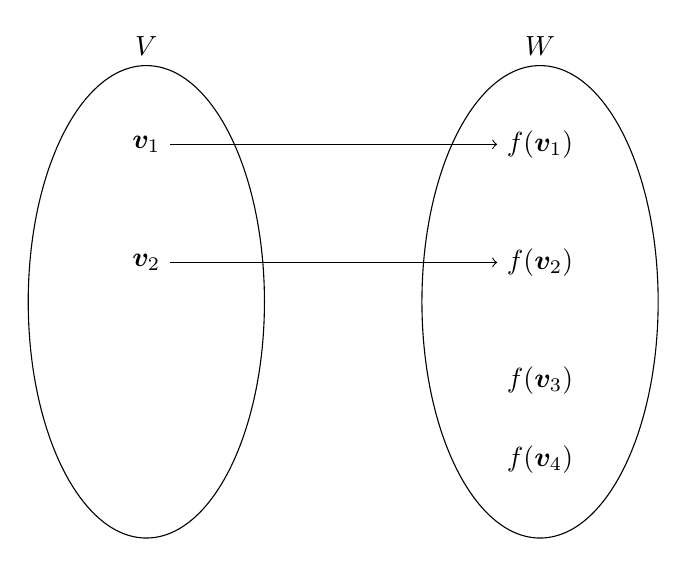
\begin{tikzpicture}
    % Draw the sets V and W
    \draw (0,0) ellipse (1.5cm and 3cm) node[above=3cm] {$V$};
    \draw (5,0) ellipse (1.5cm and 3cm) node[above=3cm] {$W$};

    % Nodes in V
    \node (v1) at (0,2) {$\bm{v}_1$};
    \node (v2) at (0,0.5) {$\bm{v}_2$};

    % Nodes in W
    \node (w1) at (5,2) {$f(\bm{v}_1)$};
    \node (w2) at (5,0.5) {$f(\bm{v}_2)$};
    \node (w3) at (5,-1) {$f(\bm{v}_3)$};
    \node (w4) at (5,-2) {$f(\bm{v}_4)$};

    % Arrows
    \draw[->] (v1) -- (w1);
    \draw[->] (v2) -- (w2);

\end{tikzpicture}
\end{center}

\vspace{0.5cm}

\noindent \textbf{Surjective}

Let \( f: V \rightarrow W \) be a linear map. We say that \( f \) is surjective or onto (or sometimes, \( f \) is a surjection) if the following holds: For all \( w \in W \), there exists a \( \bm{v} \in V \) such that \( f(\bm{v}) = w \). 

That is, any element in the codomain of \( f \) is the image of at least one element in its domain.

\begin{center}
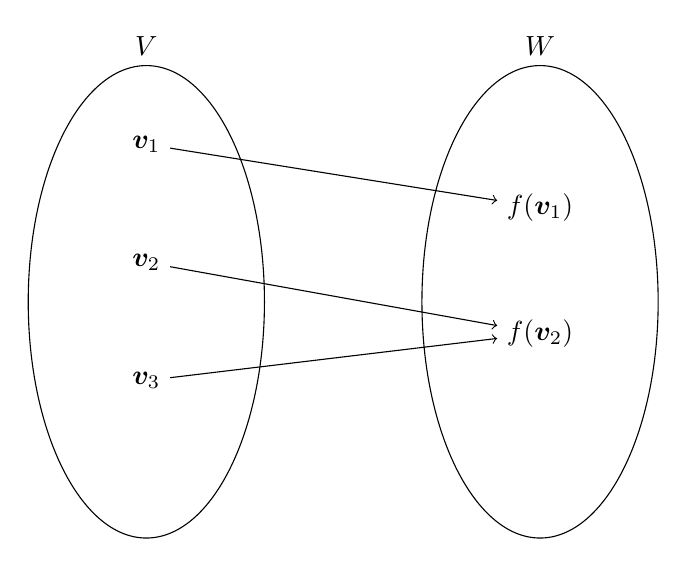
\begin{tikzpicture}
    % Draw the sets V and W
    \draw (0,0) ellipse (1.5cm and 3cm) node[above=3cm] {$V$};
    \draw (5,0) ellipse (1.5cm and 3cm) node[above=3cm] {$W$};

    % Nodes in V
    \node (v1) at (0,2) {$\bm{v}_1$};
    \node (v2) at (0,0.5) {$\bm{v}_2$};
    \node (v3) at (0, -1) {$\bm{v}_3$};


    % Nodes in W
    \node (w1) at (5,1.2) {$f(\bm{v}_1)$};
    \node (w2) at (5,-0.4) {$f(\bm{v}_2)$};

    % Arrows
    \draw[->] (v1) -- (w1);
    \draw[->] (v2) -- (w2);
    \draw[->] (v3) -- (w2);

\end{tikzpicture}
\end{center}

\noindent \textbf{Bijective}

Let \( f: V \rightarrow W \) be a linear map. We say that \( f \) is bijective (or sometimes, \( f \) is a bijection) if \( f \) is both injective and surjective. 

That is, any element in the codomain of \( f \) is the image of exactly one element in its domain. This implies that for all \( \bm{w} \in W \), there exists exactly one \( \bm{v} \in V \) such that \( f(\bm{v}) = \bm{w} \).

\begin{center}
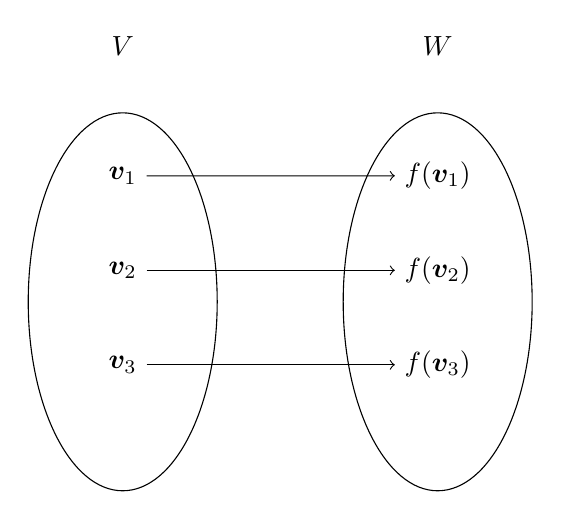
\begin{tikzpicture}[scale = 0.8]
    % Draw the sets V and W
    \draw (0,0) ellipse (1.5cm and 3cm) node[above=3cm] {$V$};
    \draw (5,0) ellipse (1.5cm and 3cm) node[above=3cm] {$W$};

    % Nodes in V
    \node (v1) at (0,2) {$\bm{v}_1$};
    \node (v2) at (0,0.5) {$\bm{v}_2$};
    \node (v3) at (0, -1) {$\bm{v}_3$};


    % Nodes in W
    \node (w1) at (5,2) {$f(\bm{v}_1)$};
    \node (w2) at (5,0.5) {$f(\bm{v}_2)$};
    \node (w3) at (5,-1) {$f(\bm{v}_3)$};

    % Arrows
    \draw[->] (v1) -- (w1);
    \draw[->] (v2) -- (w2);
    \draw[->] (v3) -- (w3);

\end{tikzpicture}
\end{center}

\vspace{0.5cm}

\noindent \textbf{Invertiblility}

A linear transformation \( T: V \rightarrow W \) is invertible if there exists a linear transformation \( S: W \rightarrow V \) such that \( S \circ T = \text{id}_V \) and \( T \circ S = \text{id}_W \), where \( \text{id}_V \) and \( \text{id}_W \) are the identity maps on \( V \) and \( W \), respectively.

Recall that linear transformations from \( \mathbb{R}^n \) to \( \mathbb{R}^m \) can be written as matrices. Thus, a matrix \( A \in M_{n \times n}(\mathbb{R}) \) is invertible if there exists a matrix \( B \in M_{n \times n}(\mathbb{R}) \) such that \( AB = BA = I_n \). Here, \( B \) is called the inverse of \( A \).

\vspace{0.5cm}

\noindent \textbf{Isomorphism}

A linear transformation \( T: V \rightarrow W \) is an isomorphism of vector spaces if \( T \) satisfies any of the following equivalent conditions:
\begin{enumerate}
    \item \( T \) is invertible.
    \item \( T \) is bijective.
\end{enumerate}
If \( T: V \rightarrow W \) is an isomorphism, we say that \( V \) and \( W \) are isomorphic vector spaces.

We can check if a linear transformation from \( \R^n \to \R^m \) is an isomorphism by checking if the determinant of the matrix representing the linear transformation is nonzero. This comes from the properties of matrix multiplication and the definition of invertibility. 

\vspace{0.5cm}

\noindent \textbf{Formula for a Plane}

The plane \( P \) in \( \mathbb{R}^3 \) determined by a point \( P_0 = (x_0, y_0, z_0) \) and a normal vector \( \bm{n} = \langle a, b, c \rangle \) is described by the equation:
\[ \bm{n} \cdot \langle x, y, z \rangle = d \]
where we set \( d = ax_0 + by_0 + cz_0 \).

\vspace{0.5cm}

\noindent \textbf{Hyperplane}

Let \( \bm{n} \in V \), with \( \bm{n} \neq 0 \). The hyperplane \( W \) normal to \( \bm{n} \) (passing through the origin) is the subspace defined as
\[ W = \{\bm{v} \in V \mid \bm{n} \cdot \bm{v} = 0\} \]
We say that \( \bm{n} \) is a normal vector of \( W \).

\section*{Quadric Surfaces}


1. Elliptic Cylinder: \( \left( \frac{x}{a} \right)^2  + \left( \frac{y}{b} \right)^2 = 1 \) 

\tikzsetnextfilename{elliptic_cylinder}
\begin{center} 
    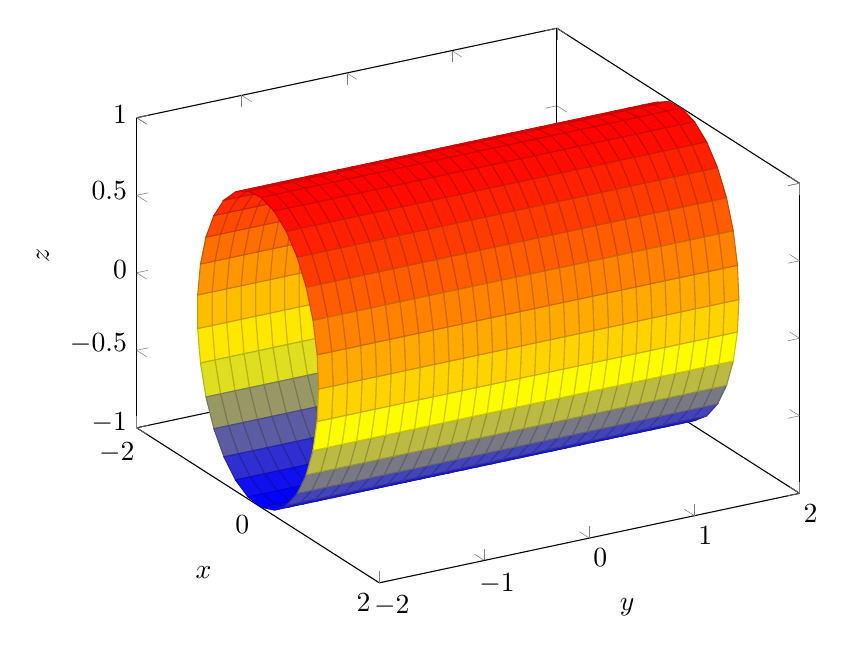
\begin{tikzpicture}
        \begin{axis}[
            view={60}{30},
            xlabel={$x$},
            ylabel={$y$},
            zlabel={$z$},
            xmin=-2, xmax=2,
            ymin=-2, ymax=2,
            zmin=-1, zmax=1,
            samples=30
        ]
    
        % Elliptic cylinder: x^2 + z^2 = 1
        \addplot3 [
            surf, 
            domain=0:360,    % Angle
            domain y=-2:2,   % Height
            z buffer=sort,
            colormap/hot
        ] 
        ({cos(x)}, y, {sin(x)}); % Parametric equation of the elliptic cylinder
    
        \end{axis}
    \end{tikzpicture}
\end{center}

2. Hyperbolic Cylinder: \( \left( \frac{y}{b} \right)^2  - \left( \frac{x}{a} \right)^2 = 1 \) 

\tikzsetnextfilename{hyperbolic_cylinder}
\begin{center}
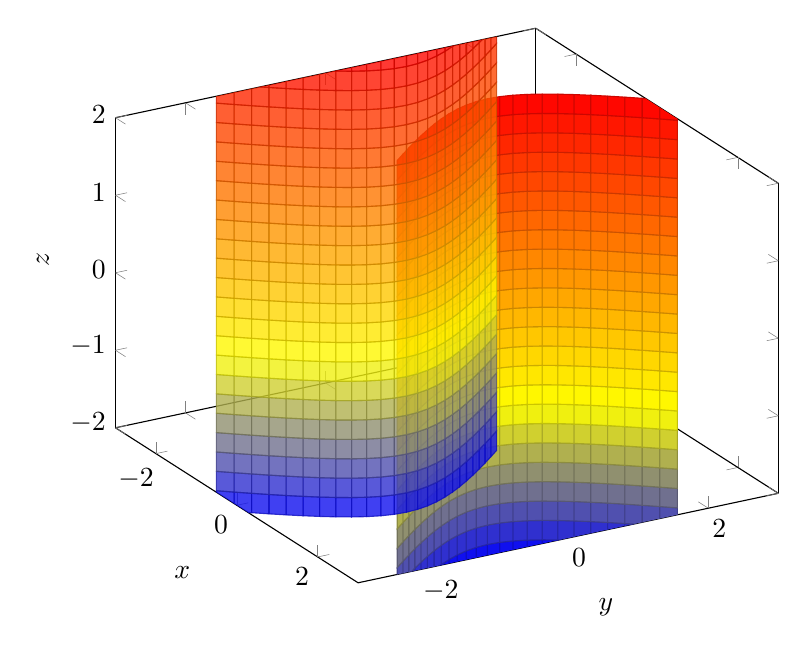
\begin{tikzpicture}
    \begin{axis}[
        view={60}{30},
        xlabel={$x$},
        ylabel={$y$},
        zlabel={$z$},
        xmin=-3, xmax=3,
        ymin=-3, ymax=3,
        zmin=-2, zmax=2,
        samples = 25
    ]

    % Hyperbolic cylinder: x^2 - z^2 = 1
    \addplot3 [
        surf, 
        domain=-2:2,    % Range for z
        domain y=-3:3,  % Range for y (hyperbola parameter)
        z buffer=sort,
        colormap/hot
    ] 
    ({sqrt(x^2 + 1)}, x, y); % Parametric equation of the hyperbolic cylinder (right branch)

    \addplot3 [
        surf, 
        domain=-2:2,    % Range for z
        domain y=-3:3,  % Range for y (hyperbola parameter)
        z buffer=sort,
        colormap/hot,
        opacity=0.8
    ] 
    ({-sqrt(x^2 + 1)}, x, y); % Parametric equation of the hyperbolic cylinder (left branch)

    \end{axis}
\end{tikzpicture}
\end{center}


3. Parabolic Cylinder: \( y = ax^2 \)

\tikzsetnextfilename{parabolic_cylinder}
\begin{center}
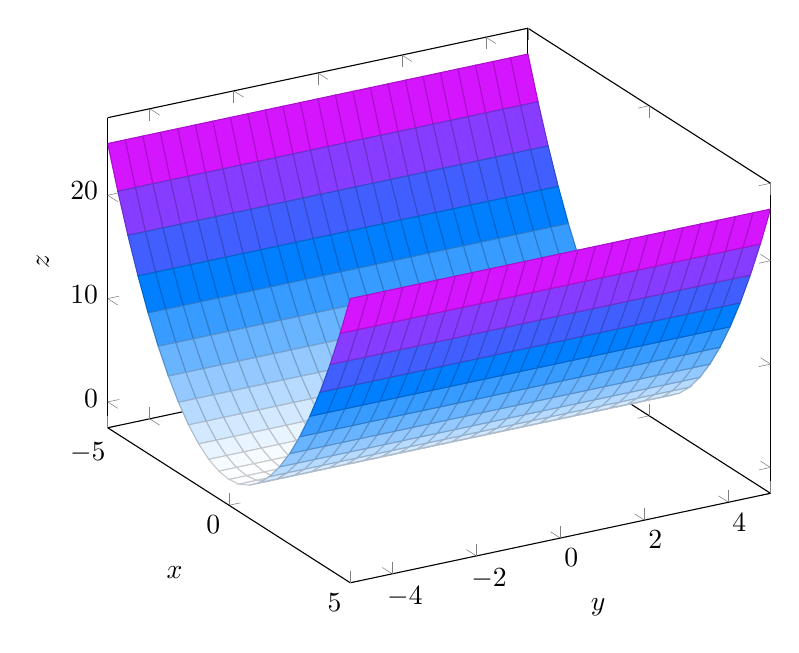
\begin{tikzpicture}
    \begin{axis}[
        view={60}{30}, % Adjusts the angle of view
        xlabel={$x$},
        ylabel={$y$},
        zlabel={$z$},
        samples=25
    ]
    
    % Parabolic Cylinder: y = x^2
    \addplot3 [
        surf,
        colormap/cool
    ]
    {x^2};
    \end{axis}
\end{tikzpicture}
\end{center}

4. Ellipsoid: \( \left( \frac{x}{a} \right)^2  + \left( \frac{y}{b} \right)^2 + \left( \frac{z}{c} \right)^2 = 1 \)

\tikzsetnextfilename{ellipsoid}
\begin{center}
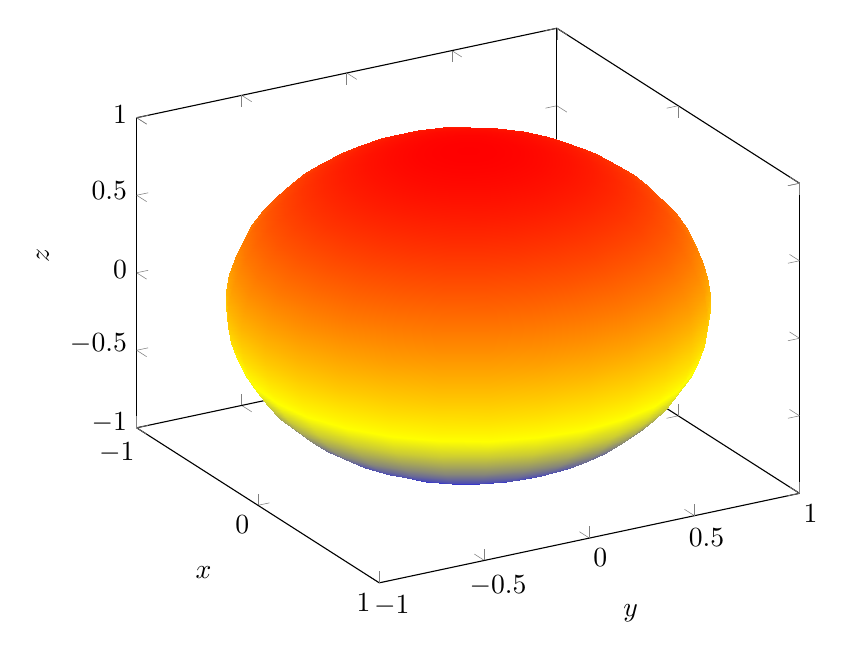
\begin{tikzpicture}
    \begin{axis}[
        view={60}{30}, % Adjust the viewing angle
        xlabel={$x$},
        ylabel={$y$},
        zlabel={$z$},
        xmin=-1, xmax=1,
        ymin=-1, ymax=1,
        zmin=-1, zmax=1,
        samples=30, % Adjust the number of samples for smoothness
        domain=0:360, % Azimuth angle (phi)
        y domain=0:180 % Polar angle (theta)
    ]

    % Sphere
    \addplot3 [
        surf, 
        shader=interp,
        colormap/hot, % You can change the colormap as needed
        z buffer=sort
    ] (
        {sin(y)*cos(x)}, 
        {sin(y)*sin(x)}, 
        {cos(y)}
    );

    \end{axis}
\end{tikzpicture}
\end{center}

5. Hyperboloid One Sheet: \(
\left( \frac{x}{a} \right)^2 + \left( \frac{y}{b} \right)^2 = \left( \frac{z}{c} \right)^2 + 1
\)

\tikzsetnextfilename{hyperboloid_one_sheet}
\begin{center}
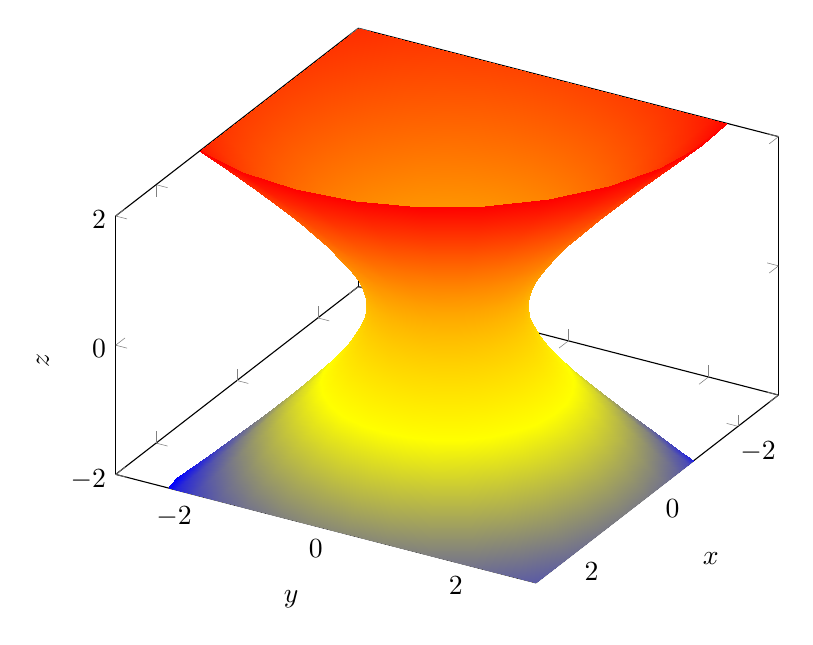
\begin{tikzpicture}
    \begin{axis}[
        view={120}{40}, % Adjust the viewing angle
        xlabel={$x$},
        ylabel={$y$},
        zlabel={$z$},
        xmin=-3, xmax=3,
        ymin=-3, ymax=3,
        zmin=-2, zmax=2,
        samples=30
    ]
    
    % Hyperboloid of one sheet
    \addplot3 [
        surf, 
        shader=interp, 
        domain=-2:2,    % u domain
        y domain=0:360, % v domain (in degrees)
        z buffer=sort,
        colormap/hot
    ] (
        {cosh(x) * cos(y)}, % x
        {cosh(x) * sin(y)}, % y
        {sinh(x)}           % z
    );

    \end{axis}
\end{tikzpicture}
\end{center}

6. Hyperboloid Two Sheets: \(
\left( \frac{x}{a} \right)^2 + \left( \frac{y}{b} \right)^2 = \left( \frac{z}{c} \right)^2 - 1
\)

\tikzsetnextfilename{hyperboloid_two_sheets}
\begin{center}
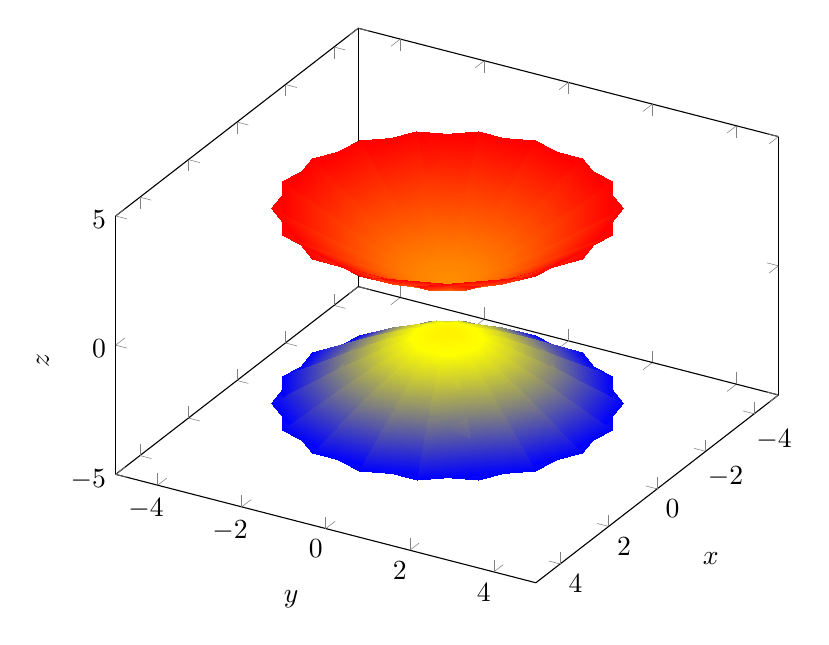
\begin{tikzpicture}
    \begin{axis}[
        view={120}{40},
        xlabel={$x$},
        ylabel={$y$},
        zlabel={$z$},
        xmin=-5, xmax=5,
        ymin=-5, ymax=5,
        zmin=-5, zmax=5,
        samples=10, % Reduced samples
    ]
    
    \addplot3 [
        surf, 
        shader=interp, 
        domain=-2:2,    % Reduced u domain
        y domain=0:360, % v domain
        z buffer=sort,
        colormap/hot
    ] (
        {sinh(x) * cos(y)}, 
        {sinh(x) * sin(y)}, 
        {cosh(x)}
    );

    \addplot3 [
        surf, 
        shader=interp, 
        domain=-2:2,    % Reduced u domain
        y domain=0:360, % v domain
        z buffer=sort,
        colormap/hot
    ] (
        {sinh(x) * cos(y)}, 
        {sinh(x) * sin(y)}, 
        {-cosh(x)}
    );

    \end{axis}
\end{tikzpicture}
\end{center}


7. Elliptic Paraboloid: \(
\left( \frac{x}{a} \right)^2 + \left( \frac{y}{b} \right)^2 = z
\)

\tikzsetnextfilename{elliptic_paraboloid}
\begin{center}
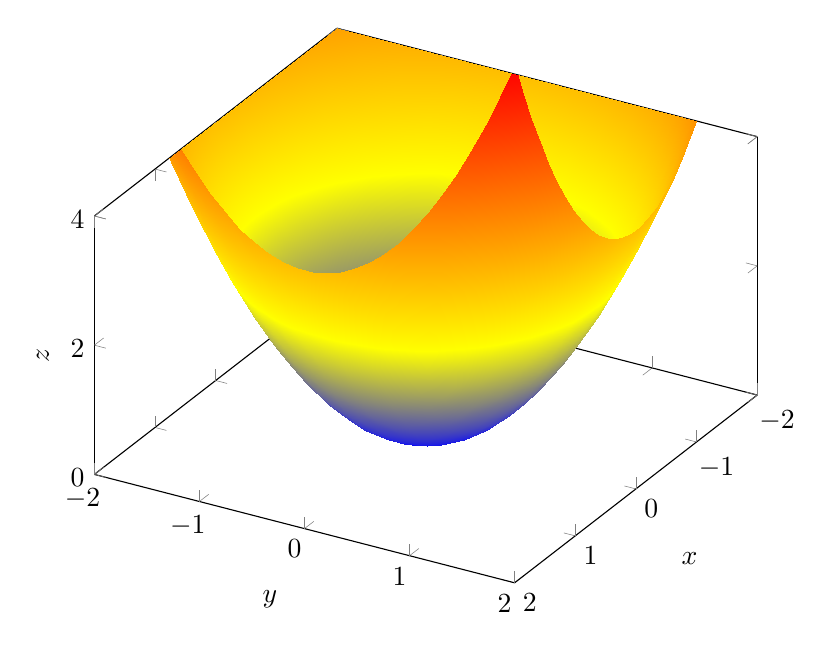
\begin{tikzpicture}
    \begin{axis}[
        view={120}{40}, % Adjust the viewing angle
        xlabel={$x$},
        ylabel={$y$},
        zlabel={$z$},
        xmin=-2, xmax=2,
        ymin=-2, ymax=2,
        zmin=0, zmax=4,
        samples=30, % Adjust for smoothness
        domain=-2:2, % x domain
        y domain=-2:2 % y domain
    ]
    
    % Elliptic Paraboloid
    \addplot3 [
        surf, 
        shader=interp, 
        z buffer=sort,
        colormap/hot
    ] (
        {x}, 
        {y}, 
        {x^2 + y^2} % Equation of the paraboloid
    );

    \end{axis}
\end{tikzpicture}
\end{center}


8.Hyperbolic Paraboloid:  \(
\left( \frac{x}{a} \right)^2 - \left( \frac{y}{b} \right)^2 = z
\)

\tikzsetnextfilename{hyperbolic_paraboloid}
\input{HyperbolicParaboloid.tex}

9. Cone (Elliptical): \(
\left( \frac{x}{a} \right)^2 + \left( \frac{y}{b} \right)^2 = \left( \frac{z}{c} \right)^2
\)

\tikzsetnextfilename{cone}
\begin{center}
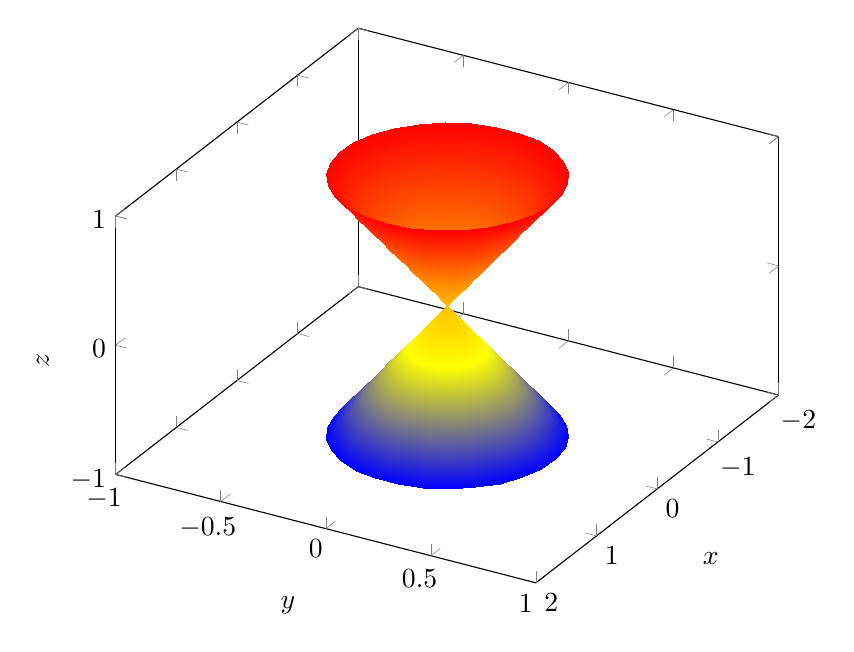
\begin{tikzpicture}
    \begin{axis}[
        view={120}{40}, % Adjust the viewing angle
        xlabel={$x$},
        ylabel={$y$},
        zlabel={$z$},
        xmin=-2, xmax=2,
        ymin=-1, ymax=1,
        zmin=-1, zmax=1,
        samples=30, % Adjust for smoothness
        domain=0:360, % theta domain (in degrees)
        y domain=-1:1 % z domain
    ]
    
    % Elliptic Cone
    \addplot3 [
        surf, 
        shader=interp, 
        z buffer=sort,
        colormap/hot
    ] (
        {y * cos(x)}, % x, scaling factor for ellipse in x direction
        {0.5 * y * sin(x)}, % y, scaling factor for ellipse in y direction
        {y}           % z
    );

    \end{axis}
\end{tikzpicture}
\end{center}

\vspace{1cm}

\noindent \textbf{Graphs}

Given a function \( f : \mathbb{R}^n \rightarrow \mathbb{R} \), its graph is the following subset of \( \mathbb{R}^{n+1} \):
\[ \Gamma_f := \{ (x_1, \dots, x_n, f(x_1, \dots, x_n)) \} \subset \mathbb{R}^{n+1} \]
In other words, the graph is given by the equation
\[ x_{n+1} = f(x_1, \dots, x_n) \] in \( \mathbb{R}^{n+1} \).

\vspace{0.5cm}


\noindent \textbf{Traces}

The trace in the plane \( P \) of a graph \( \Gamma \subset \mathbb{R}^3 \) is the intersection of \( \Gamma \)
with \( P \). That is,
\[ \Gamma \cap P = \{ x \in \mathbb{R}^3 \mid x \in \Gamma \text{ and } x \in P \} \]


\vspace{0.5cm}

\noindent \textbf{Level Curves}

The level curves (isoclines, contour map) of a function of two variables \( f(x, y) \) are the \( z \)-traces of the graph \( z = f(x, y) \).


\vspace{0.5cm}

\noindent \textbf{Vanishing Locus}

Given a multivariable function \( G(x_1, \dots, x_n) : \mathbb{R}^n \rightarrow \mathbb{R} \), its vanishing
locus is the set of points
\[ \{ (x_1, \dots, x_n) \mid G(x_1, \dots, x_n) = 0 \} \]

All quadric surfaces are the vanishing loci of the general quadratic equation
\[ Q(x, y, z) = Ax^2 + By^2 + Cz^2 + Dxy + Exz + Fyz + ax + by + cz + d \]



\section*{Limits}

\noindent \textbf{Limit of Sequence Definition}

Let $\{\bm{a_n}\}$ be a sequence of vectors in $\mathbb{R}^k$. We say that the sequence $\{\bm{a_n}\}$ converges to the vector $\bm{L} \in \mathbb{R}^k$ if the following holds:

\begin{quote}
    For all $\varepsilon > 0$, there exists an $M$ such that for all $m > M$, $\left\|\bm{a_m} - \bm{L}\right\| < \varepsilon$.
\end{quote}

We say $\bm{L}$ is the \textit{limit} of the sequence $\{\bm{a_n}\}$. If no such $\bm{L}$ exists, we say that $\{\bm{a_n}\}$ \textit{diverges}.

\vspace{0.5cm}

\noindent \textbf{Definition of a Ball}

Let $P \in \R^n$. The open ball of radius $\varepsilon$ around $P$, denoted $B_{\varepsilon}(P)$, is the set of points defined by
\[ B_{\varepsilon}(P) := \{ \bm{x} \in \R^n \,|\, \|\bm{x} - \bm{P}\| < \varepsilon \}. \]

\vspace{0.5cm}

\noindent \textbf{Subsequences}

Let $\{\bm{a_n}\}$ be a sequence of vectors in $\R^k$. A subsequence of $\{\bm{a_n}\}$ is a sequence $\{\bm{b_i}\}$, where
\[\bm{b_i} = \bm{a_{n_i}}\]
such that $n_1 < n_2 < \cdots < n_i < \cdots$.

Let $\{\bm{a_n}\}$ be a sequence of vectors in $\R^k$. If $\{\bm{a_n}\}$ has a subsequence $\{\bm{a_{n_i}}\}$ that diverges, then $\{\bm{a_n}\}$ diverges.

\vspace{0.5cm}

\noindent \textbf{Delta-Epsilon Limit Definition}

A function \( f : \R^n \rightarrow \R^m \) has the limit \( \bm{b} \) at \( \bm{a} \) if the following holds:
\begin{quote}
    For all \(\varepsilon > 0\), there exists \(\delta > 0\) such that for all \( \bm{x} \in \R^n \),\\
    \(0 < \|\bm{x} - \bm{a}\| < \delta\) implies \(\|f(\bm{x}) - \bm{b}\| < \varepsilon\).
\end{quote}

\vspace{0.5cm}

\noindent \textbf{Properties of Limits of a function from \( \R^n \to \R \)}

Let \( f, g : \mathbb{R}^n \rightarrow \mathbb{R} \) be functions of \( n \) variables. Suppose that \(\lim_{\bm{x} \to \bm{P}} f(\bm{x})\) and \(\lim_{\bm{x} \to \bm{P}} g(\bm{x})\) exist. Then

\begin{enumerate}
    \item[{\bf a.}] Sum Law:
    \[\lim_{\bm{x} \to \bm{P}} (f(\bm{x}) + g(\bm{x})) = \lim_{\bm{x} \to \bm{P}} f(\bm{x}) + \lim_{\bm{x} \to \bm{P}} g(\bm{x})\]
    
    \item[{\bf b.}] Scalar Multiple Law:
    \[\lim_{\bm{x} \to \bm{P}} \lambda f(\bm{x}) = \lambda \lim_{\bm{x} \to \bm{P}} f(\bm{x})\]
    
    \item[{\bf c.}] Product Law:
    \[\lim_{\bm{x} \to \bm{P}} (f(\bm{x})g(\bm{x})) = \left( \lim_{\bm{x} \to \bm{P}} f(\bm{x}) \right)\left( \lim_{\bm{x} \to \bm{P}} g(\bm{x}) \right)\]
    
    \item[{\bf d.}] Quotient Law: If \(\lim_{\bm{x} \to \bm{P}} g(\bm{x}) \neq 0\),
    \[\lim_{\bm{x} \to \bm{P}} \frac{f(\bm{x})}{g(\bm{x})} = \frac{\lim_{\bm{x} \to \bm{P}} f(\bm{x})}{\lim_{\bm{x} \to \bm{P}} g(\bm{x})}\]
\end{enumerate}

\vspace{0.5cm}

\noindent \textbf{Limit Point}

Let \( X \subset \mathbb{R}^n \). We say that a point \( p \in \mathbb{R}^n \) is a \textit{limit point} of \( X \) if there is a sequence \( \{a_n\} \) contained inside \( X \) such that \( \{a_n\} \) converges to \( p \).

\vspace{0.5cm}

\noindent \textbf{Paths to show a limit does not exist}

Let \( X \subset \mathbb{R}^n \), let \( f : X \rightarrow \mathbb{R}^m \) be a function, and let \( a \) be a limit point of \( X \). Then the following statements are equivalent:
\begin{enumerate}
    \item[\textbf{a.}] \(\lim_{\bm{x} \to \bm{a}} f(\bm{x}) = \bm{b}\)
    
    \item[\textbf{b.}] For every sequence \(\{\bm{a_n}\}\) converging to \(\bm{a}\) (with \(\bm{a_n} \neq \bm{a}\)), the sequence \(\{f(\bm{a_n})\}\) converges to \(\bm{b}\).
\end{enumerate}
In other words, in order for a limit of a multivariable function to exist, it must yield the same value along all possible approaches.


\vspace{0.5cm}

\noindent \textbf{Squeeze Theorem}

Let \( f(\bm{x}) \), \( g(\bm{x}) \), and \( h(\bm{x}) \) be functions of \( n \) variables such that 
\[\lim_{\bm{x} \to \bm{P}} f(\bm{x}) = L = \lim_{\bm{x} \to \bm{P}} h(\bm{x}).\]
If there exists \(\delta > 0\) such that for all \( \bm{x} \in B_{\delta}(\bm{P}) \setminus \{\bm{P}\} \), we have that 
\[f(\bm{x}) \leq g(\bm{x}) \leq h(\bm{x}).\]

\vspace{0.5cm}

\noindent \textbf{Limits using Polar Coordinates}

Let \( f(x, y) : \mathbb{R}^2 \rightarrow \mathbb{R} \) be a function of two variables, which we can express in polar coordinates as \( g(r, \theta) := f(r \cos(\theta), r \sin(\theta)) \). Then 
\[\lim_{(x,y) \to (0,0)} f(x,y) = L\]
if and only if there exists \(\delta > 0\) and a function \( h : \mathbb{R} \rightarrow \mathbb{R} \) such that
\begin{enumerate}
    \item If \(0 < r < \delta\), then \(\left| g(r,\theta) - L \right| \leq h(r)\) for all \(\theta\), \textbf{AND}
    \item \(\lim_{r \to 0} h(r) = 0\).
\end{enumerate}

\textbf{Corollary 2.3.14.} If \(\lim_{r \to 0} g(r,\theta)\) depends on \(\theta\), then the value of the limit will differ for different straight line paths. Thus, \(\lim_{(x,y) \to (0,0)} f(x,y)\) does not exist.

\vspace{1cm}

\section*{Derivatives}

\noindent \textbf{Limit Definition of the Derivative}

A multivariable function \( f : A \subset \mathbb{R}^m \rightarrow \mathbb{R}^n \) is \textit{differentiable} at an interior point \( \bm{x_0} \) of \( A \) if there exists a linear transformation \( T : \mathbb{R}^m \rightarrow \mathbb{R}^n \) such that
\[\lim_{\bm{h} \to \bm{0}} \frac{\|f(\bm{x_0} + \bm{h}) - f(\bm{x_0}) - T(\bm{h})\|}{\|\bm{h}\|} = 0.\]
The derivative of \( f \) at \( \bm{x_0} \) is the linear transformation \( Df(\bm{x_0}) := T \). By our characterization of linear transformations, \( Df(\bm{x_0}) : \mathbb{R}^m \rightarrow \mathbb{R}^n \) corresponds to a matrix \([Df(\bm{x_0})] \in M_{n \times m}(\mathbb{R})\).

\vspace{0.5cm}

\noindent \textbf{Chain Rule}

Let \( f : \mathbb{R}^n \rightarrow \mathbb{R}^m \), and let \( g : \mathbb{R}^m \rightarrow \mathbb{R}^k \) be multivariable functions such that \( f \) is differentiable at \( \bm{x_0} \in \mathbb{R}^n \), and \( g \) is differentiable at \( f(\bm{x_0}) \in \mathbb{R}^m \). Then \( g \circ f : \mathbb{R}^n \rightarrow \mathbb{R}^k \) is differentiable at \( \bm{x_0} \in \mathbb{R}^n \), and
\[ D(g \circ f)(\bm{x_0}) = Dg(f(\bm{x_0})) \circ Df(\bm{x_0}) \]
We can prove this using the definition of the derivative. However, since we know that the derivative can be computed in terms of the Jacobian, we equivalently have

\vspace{0.25cm}

\textit{In Coordinates: } Suppose that \( f : \mathbb{R}^n \rightarrow \mathbb{R}^m \) is differentiable at \( \bm{x_0} \in \mathbb{R}^n \), and \( g : \mathbb{R}^m \rightarrow \mathbb{R}^k \) is differentiable at \( f(\bm{x_0}) \in \mathbb{R}^m \). Then
\[ [J_{g \circ f} (\bm{x_0})] = [J_g(f(\bm{x_0}))] [J_f (\bm{x_0})] \]

\vspace{0.25cm}

\textit{For Paths:} Let \( f(x_1, \ldots, x_n) : \mathbb{R}^n \rightarrow \mathbb{R} \) be a differentiable function, and let \( \bm{r}(t) = \langle x_1(t), \ldots, x_n(t) \rangle : \mathbb{R} \rightarrow \mathbb{R}^n \) be a vector-valued function. Then \( f(\bm{r}(t)) : \mathbb{R} \rightarrow \mathbb{R} \) is a single-variable function, and the derivative of \( f \) at \( t_0 \) along the path \( \bm{r}(t) \) is given by
\[
\frac{d}{dt} f(\bm{r}(t_0)) = \sum_{i=1}^{n} \frac{\partial f}{\partial x_i}(\bm{r}(t_0)) x'_i(t_0)
\]
where \( x'_i(t_0) \) is the derivative of the \( i \)-th component of \( \bm{r}(t) \) at \( t_0 \). This measures the rate of change of \( f \) along the path \( \bm{r}(t) \).

\[ f(\mathbf{r}(t_0)) = \nabla f(\mathbf{r}(t_0)) \cdot \mathbf{r}'(t_0) \]


\vspace{0.5cm}

\noindent \textbf{The Jacobian}


Let \( f : A \subset \R^m \rightarrow \R^n \) be a multivariable function defined by \( f^i : A \subset \R^m \rightarrow \R \):
\[
f(\bm{x}) =
\begin{bmatrix}
    f^1(\bm{x}) \\
    \vdots \\
    f^n(\bm{x})
\end{bmatrix}.
\]
The Jacobian matrix of \( f \) at \( \bm{x_0} \) is
\[
[J_f (\bm{x_0})] =
\begin{bmatrix}
    D_1f^1(\bm{x_0}) & D_2f^1(\bm{x_0}) & \cdots & D_mf^1(\bm{x_0}) \\
    D_1f^2(\bm{x_0}) & D_2f^2(\bm{x_0}) & \cdots & D_mf^2(\bm{x_0}) \\
    \vdots & \vdots & \ddots & \vdots \\
    D_1f^n(\bm{x_0}) & D_2f^n(\bm{x_0}) & \cdots & D_mf^n(\bm{x_0})
\end{bmatrix}
\]
if the partial derivatives exist.



\vspace{0.5cm}

\noindent \textbf{Directional Derivative}

If \( \mathbf{u} = \langle u_1, \ldots, u_n \rangle \) is a unit vector in \( \mathbb{R}^n \), then the directional derivative of a function \( f \) at the point \( \mathbf{x_0} \in \mathbb{R}^n \) in the direction of \( \mathbf{u} \) is defined as
\[ D_{\mathbf{u}}f(\mathbf{x_0}) = u_1 \frac{\partial f}{\partial x_1}(\mathbf{x_0}) + \cdots + u_n \frac{\partial f}{\partial x_n}(\mathbf{x_0}). \]

\vspace{0.5cm}

\noindent \textbf{Gradient}

If \( f(x_1, \ldots, x_n) \) is a function of \( n \) variables, then the \textit{gradient} of \( f \) is the vector-valued function given by
\[ \nabla f = \left\langle \frac{\partial f}{\partial x_1}, \ldots, \frac{\partial f}{\partial x_n} \right\rangle. \]

That is, \( \nabla f \) is the transpose of the matrix of partial derivatives of \( f \),
\[ \nabla f = \begin{bmatrix} D(f\left(\bm{x_0}\right)) \end{bmatrix}^{\top}, \]

where \( [A]^{\top} \) indicates the transpose matrix.

Thinking of \( z \) as the height of \( z = f(x,y) \), the gradient \( \nabla f \) points in the direction of steepest ascent. 

The opposite of the gradient, \( -\nabla f \), points in the direction of steepest descent.

\vspace{0.5cm}

\noindent \textbf{Linear Approximation}

If \( f : A \subset \mathbb{R}^m \rightarrow \mathbb{R} \) is differentiable at a point \( \bm{a} = (a_1, \ldots, a_n) \), and \( \bm{x} = (x_1, \ldots, x_n) \) is close to \( \bm{a} \), then
\begin{align*}
f(\bm{x}) &\approx f(\bm{a}) + \begin{bmatrix} D_1f(\bm{a}) & D_2f(\bm{a}) & \cdots & D_nf(\bm{a}) \end{bmatrix} (\bm{x} - \bm{a}) \\
         &= f(\bm{a}) + \sum_{i=1}^{n} \left( \frac{\partial f}{\partial x_i}(\bm{a}) \right) (x_i - a_i).
\end{align*}



\vspace{0.5cm}

\noindent \textbf{Critical Point}

A point \( \bm{P} \in \mathbb{R}^n \) is said to be a \textit{critical point} of a function \( f : \mathbb{R}^n \rightarrow \mathbb{R} \) if either
\begin{enumerate}
    \item[\textbf{a.}] \( Df(\bm{P}) = 0 \), \textbf{OR}
    \item[\textbf{b.}] \( Df(\bm{P}) \) does not exist.
\end{enumerate}


\vspace{0.5cm}

\noindent \textbf{Hessian Matrix}

The Hessian matrix of \( f : \R^n \rightarrow \R \) at \( \bm{x_0} \) is
\[
[H_f (\bm{x_0})] =
\begin{bmatrix}
    D_1D_1f(\bm{x_0}) & D_2D_1f(\bm{x_0}) & \cdots & D_nD_1f(\bm{x_0}) \\
    D_1D_2f(\bm{x_0}) & D_2D_2f(\bm{x_0}) & \cdots & D_nD_2f(\bm{x_0}) \\
    \vdots & \vdots & \ddots & \vdots \\
    D_1D_nf(\bm{x_0}) & D_2D_nf(\bm{x_0}) & \cdots & D_nD_nf(\bm{x_0})
\end{bmatrix},
\]
where \( D_iD_jf(\bm{x_0}) \) denotes the second partial derivative of \( f \) with respect to \( x_i \) and then \( x_j \) at \( \bm{x_0} \).


\vspace{0.5cm}

\noindent \textbf{Clairaut's Theorem.} 

Let \( f : \mathbb{R}^n \rightarrow \mathbb{R} \). Suppose that \( D_i f \), \( D_j f \), and \( D_i D_j f \) exist and are continuous on an open disk \( D \subset \mathbb{R}^n \). Then \( D_j D_i f \) exists on \( D \), and moreover, \( D_i D_j f = D_j D_i f \) on the disk \( D \).


\vspace{0.5cm}

\noindent \textbf{Second Derivative Test}

Let \( \bm{x_0} \subset U \) be a critical point of \( f(x, y) : U \rightarrow \mathbb{R} \), and suppose that \( f \) is in \( C^2(U) \). Let us write \( D = \det[H_f (\bm{x_0})] \). 
\begin{enumerate}
    \item[\textbf{a.}] If \( D > 0 \) and \( f_{xx}(\bm{x_0}) > 0 \), then there is a local minimum at \( \bm{x_0} \).
    \item[\textbf{b.}] If \( D > 0 \) and \( f_{xx}(\bm{x_0}) < 0 \), then there is a local maximum at \( \bm{x_0} \).
    \item[\textbf{c.}] If \( D < 0 \), then \( f \) has a saddle point at \( \bm{x_0} \).
    \item[\textbf{d.}] If \( D = 0 \) or does not exist, then the test is inconclusive.
\end{enumerate}

\vspace{0.5cm}

\noindent \textbf{Convex Subset}

A subset \(A \subset \R^n\) is said to be a convex subset of \(\R^n\) if it contains the line segment joining any two points of \(A\). That is, for all \(\bm{a}, \bm{b} \in A\), and for all \(t \in [0, 1]\), then \(\bm{a} + t(\bm{b} - \bm{a}) \in A\).


\vspace{0.5cm}


\noindent \textbf{Bounded}

A subset \( D \subset \mathbb{R}^n \) is \textit{bounded} if there exists some \( r > 0 \) such that
\[ D \subset B_r(\bm{0}). \]

\vspace{0.5cm}

\noindent \textbf{Boundary Point}

A point \( \bm{x_0} \in \mathbb{R}^n \) is a \textit{boundary point} of \( D \subset \mathbb{R}^n \) if: for all \( \varepsilon > 0 \),
\begin{enumerate}
    \item[\textbf{a.}] \( B_{\varepsilon}(\bm{x_0}) \cap D \) is non-empty, and
    \item[\textbf{b.}] \( B_{\varepsilon}(\bm{x_0}) \cap D^c \) is non-empty,
\end{enumerate}
where \( D^c \) is the complement of \( D \) in \( \mathbb{R}^n \).

A subset \( D \subset \mathbb{R}^n \) is \textit{closed} if it contains all of its boundary points.

\vspace{0.5cm}


\noindent \textbf{Langrange Multipliers}

Assume that \( f(x,y) \) and \( g(x,y) \) are differentiable functions. If
\begin{enumerate}
    \item[\textbf{a.}] \( f(x, y) \) has a local maximum or minimum subject to the constraint \( g(x, y) = 0 \) at a point \( (a, b) \), \textbf{AND}
    \item[\textbf{b.}] \( \nabla g(a, b) \neq 0 \)
\end{enumerate}
then there is a scalar \( \lambda \) such that
\[ \nabla f(a, b) = \lambda \nabla g(a, b). \]

We can use the Lagrange equations
\[ f_x(a, b) = \lambda g_x(a, b) \] and \[ f_y(a, b) = \lambda g_y(a, b). \]


\vspace{0.5cm}

\noindent \textbf{Global Max/Min}

If \( D \) is a closed and bounded subset of \( \mathbb{R}^n \), and \( f \) is a continuous function on \( D \), then \( f \) has a global maximum and a global minimum in \( D \). That is, there exists an \( M \in D \) and an \( m \in D \) such that 
\[ f(m) \leq f(x) \leq f(M) \]
for all \( x \in D \).

\vspace{0.75cm}

\section*{Frenet Frame Formulas}

$$\bm{T}(t) = \frac{1}{||\bm{r}'(t)||}\bm{r}'(t)$$

$$\bm{N}(t) = \frac{1}{||\bm{T}'(t)||}\bm{T}'(t)$$

$$\bm{B} = \bm{T} \times \bm{N}$$

$$\bm{B}(t) = \frac{\bm{r}'(t) \times \bm{r}''(t)}{\left| \left| \bm{r}'(t) \times \bm{r}''(t)\right| \right|}$$

$$\bm{N} = \bm{B} \times \bm{T}$$

$$\kappa(t) = \frac{1}{||\bm{r}'(t)||}||\bm{T}'(t)||$$

$$\kappa(t) = \frac{||\bm{r}'(t) \times \bm{r}''(t)||}{||\bm{r}'(t)||^3}$$

$$\kappa(t) = \frac{1}{R}$$

\end{document}
